%%%%%%%%%%%%%%%%%%%%%%%%%%%%%%%%%%%%%%%%%%%%%%%%%%%%%%
%%%%%%%%%%%%%%%%%%%%%%%%%%%%%%%%%%%%%%%%%%%%%%%%%%%%%%%%%%%%%%%%%%%%
\def\scl{1}%scaling factor of the picture

\def\hauteur{0.35}% de l'axe des roues
\tikzset{
  roue/.pic={
    \fill[black!20!gray!70!] (0, \hauteur) circle (0.35 cm);
    \fill[gray!20!] (0, \hauteur) circle (0.31 cm);
    \fill[black!20!gray!70!] (0, \hauteur) circle (0.28 cm);


  \fill[color=gray,draw=gray!20!, ultra thin] %,rotate=45
 (0.1, \hauteur + -0.1) rectangle (-0.1, \hauteur + 0.1);
    \fill[color=gray,draw=gray!20!, ultra thin] (0, \hauteur) circle (0.08 cm);

  \fill[color=gray,draw=gray!20!, ultra thin] %,rotate=45
 (0.08, \hauteur + 0.12) rectangle (-0.08, \hauteur + 0.18);

  \fill[color=gray,draw=gray!20!, ultra thin] %,rotate=45
 (0.1, \hauteur + 0.2) rectangle (-0.1, \hauteur + 0.35);

  %\fill[color=gray,draw=gray!20!, ultra thin] (0.1, 0.9) rectangle (17.4, 2.2);
  %\fill[color=gray,draw=gray!20!, ultra thin] (0.1, 0.9) rectangle (17.4, 2.2);



  }
}


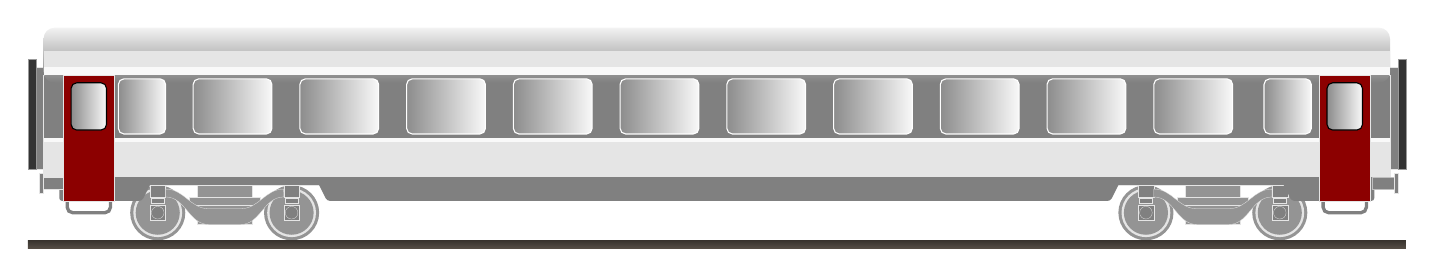
\begin{tikzpicture}[
  scale=\scl,
  %wagon/.style={yellow!30!brown!20!,rounded corners,draw=black,thick},
  wagon/.style={green!70!brown!20!black!75!,draw=black,thick},
 % toit/.style={black!70!brown!20!,draw=gray,thick},
  %roue/.style={brown!20!black!70!,draw=black,thick},
  fenetre/.style={white,rounded corners = 2pt,draw=black, thick},
  porte/.style={red!55!black,draw=gray!20!, ultra thin}
  ]

  \begin{scope}[xshift=0 cm,yshift=0 cm]
%
%         LIAISONS
%
  \fill[color=gray,draw=gray!20!, ultra thin] % 
 (0.1, 0.9) rectangle (17.4, 2.2);

  \fill[color=black!80!,draw=gray!80!, ultra thin] % 
 (0, 0.9) rectangle (0.1, 2.3);
  \fill[color=black!80!,draw=gray!80!, ultra thin] % 
 (17.4, 0.9) rectangle (17.5, 2.3);

%
%     CORPS DU WAGON
%

  \fill[color=gray,draw=gray!20!, ultra thin] % 
 (0.2, 0.7) rectangle (17.3, 2.1);

  \shade[bottom color=gray, top color=gray!10!, rounded corners]  % toit
 (0.2, 2) rectangle (17.3, 2.7);
  \fill[color=gray!20!] % gris clair
 (0.2, 2.1) rectangle (17.3, 2.4);
  \fill[color=gray!20!] % gris clair
 (0.2, 0.8) rectangle (17.3, 1.25);
  \fill[color=gray!5!] % blanc
 (0.2, 2.1) rectangle (17.3, 2.2);
  \fill[color=gray!5!] % blanc
 (0.2, 1.25) rectangle (17.3, 1.3);

%  ROUES
  \pic at (1.65,0)    {roue};
  \pic at (3.35,0)    {roue};
  \pic at (14.2,0)    {roue};
  \pic at (15.9,0)    {roue};
 % ESSIEUX
\def\y{0.2}
  \foreach \x in {2.5, 15.05}
   {
 \fill[black!20!gray!70!,draw=gray!20!, ultra thin] 
  (\x - 0.35, 0.2) rectangle (\x + 0.35, 0.45);

 \fill[black!20!gray!70!,draw=gray!20!, ultra thin] 
  (\x - 0.45, 0.45) rectangle (\x + 0.45, 0.55);

 \fill[black!20!gray!70!,draw=gray!20!, ultra thin] 
  (\x - 0.35, 0.55) rectangle (\x + 0.35, 0.7);

    \coordinate (A) at (\x + -0.75,\y + 0.45) ;
      \coordinate (B) at (\x - 0.2,\y + 0.2) ;
      \coordinate (C) at (\x + 0.2,\y + 0.2) ;
    \coordinate (D) at (\x + 0.75,\y + 0.45) ;
    \coordinate (E) at (\x + 0.75,\y + 0.35) ;
      \coordinate (F) at (\x + 0.2,\y + 0) ;
      \coordinate (G) at (\x - 0.2,\y + 0) ;
    \coordinate (H) at (\x - 0.75,\y + 0.35) ;
 \fill[black!20!gray!70!,draw=gray!20!, ultra thin] 
    (A) to[out=0,in=180] (B) to[out=0,in=180] (C) to[out=0,in=180]
    (D) to[out=-90,in=90] (E) to[out=180,in=0] (F) to[out=180,in=0]
    (G) to[out=180,in=0] (H) -- cycle;
  }

% BAS DE CAISSE
  \coordinate (A) at (0.4,0.8) ;
      \coordinate (B) at (17.1,0.8) ;

      \coordinate (C) at (17.1,0.5) ;
      \coordinate (D) at (16.05,0.5) ;

      \coordinate (E) at (15.9,0.8) ;
      \coordinate (F) at (13.9,0.8) ;

      \coordinate (G) at (13.75,0.5) ;
      \coordinate (H) at (3.8,0.5) ;

      \coordinate (I) at (3.65,0.8) ;
      \coordinate (J) at (1.60,0.8) ;

      \coordinate (K) at (1.45,0.5) ;
    \coordinate (L) at (0.4,0.5) ;

  \fill[color=gray, rounded corners=1pt] % gris Foncé
    (A) -- (B) -- (C) -- (D) -- (E) -- (F) -- (G) -- (H) -- (I) -- (J) --
 (K) -- (L) -- cycle;


 % BUTOIR gauche  
  \fill[color=gray,draw=gray!20!, ultra thin] % 
 (0.2, 0.65) rectangle (0.5, 0.8);
  \fill[color=gray,draw=gray!20!, ultra thin] % 
 (0.15, 0.6) rectangle (0.2, 0.85);
 % BUTOIR droite  
  \fill[color=gray,draw=gray!50!, ultra thin] % 
 (17.07, 0.65) rectangle (17.35, 0.8);
  \fill[color=gray,draw=gray!20!, ultra thin] % 
 (17.35, 0.6) rectangle (17.4, 0.85);

      % FENÊTRES
  \foreach \t in {0, 1,..., 9}
  \shade[bottom color=gray!5!, top color=gray!90!, shading angle={90},rounded corners=2pt, draw=white]
   (2.1 + 1.35556*\t, 1.35) rectangle (3.1 + 1.35556*\t, 2.05);
  \foreach \t in {0, 14.55}
  \shade[bottom color=gray!5!, top color=gray!90!, shading angle={90},rounded corners=2pt, draw=white]
   (1.15 + \t, 1.35) rectangle (1.75 + \t, 2.05);


      % PORTES
    \draw[rounded corners = 2pt,draw=gray,very thick] % marche
 (0.5, 0.35) rectangle (1.05, 0.6);
    \draw[rounded corners = 2pt,draw=gray,very thick] % marche
 (16.45, 0.35) rectangle (17, 0.6);

    \fill[porte]
 (0.45, 0.5) rectangle (1.1, 2.1);
    \fill[porte]
 (16.4, 0.5) rectangle (17.05, 2.1);

  \foreach \t in {0.55, 16.5} % fenêtre
  \shade[bottom color=gray!5!, top color=gray!90!, shading angle={90},rounded corners=2pt, draw=black]
   (\t, 1.4) rectangle (0.45 + \t, 2);

  % RAIL
  \shade[bottom color=brown!20!gray!60!black, top color=brown!20!gray!40!black]
 (0, 0) rectangle (17.5, -0.1);

  \end{scope}
%
%
\end{tikzpicture}
%
